\documentclass[english]{thesis}
\usepackage[cpp]{mypackage}
\usepackage{hyperref}

\title{Homework 6}
\school{School of Data and Computer Science}
\author{Hongzheng Chen}
\stunum{17341015}
\headercontext{Parallel and Distributed Computing}

\begin{document}

\maketitle

\section{Problem 1}
Start from the provided skeleton code \verb'error-test.cu' that provides some convenience macros for error checking.
The macros are defined in the header file \verb'error_checks_1.h'.
Add the missing memory allocations and copies and the kernel launch and check that your code works.
\begin{enumerate}
\item What happens if you try to launch kernel with too large block size?
When do you catch the error if you remove the \verb'cudaDeviceSynchronize()' call?
\item What happens if you try to dereference a pointer to device memory in host code?
\item What if you try to access host memory from the kernel?
Remember that you can use also cuda-memcheck!
\item If you have time, you can also check what happens if you remove all error checks and do the same tests again.
\end{enumerate}

\bigskip
\textit{Answer.} The code is in \verb'error-test.cu', and the result is shown below.
\begin{figure}[H]
\centering
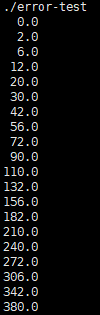
\includegraphics[width=0.2\linewidth]{fig/res1.PNG}
\end{figure}

\begin{enumerate}
	\item The maximum block size of my GPU is 1024 (threads), and I request 2048 threads, which results in the following error.
\begin{lstlisting}[language=bash]
Error: vector_add kernel at error-test.cu(50): invalid configuration argument
\end{lstlisting}
	Well, even I comment the \verb'cudaDeviceSynchronize()', the error is still caught after the \verb'vectorAdd' function, and the reported error is the same.
	\item It will cause a segment fault, since the memory is not allocated on the host.
	\item It will cause an illegal memory access, since the memory is not allocated on the device. Error as shown below.
\begin{lstlisting}[language=bash]
Error: vector_add kernel at error-test.cu(53): an illegal memory access was encountered
\end{lstlisting}
	\item For 1 and 3, the program runs as usual and no errors will be reported.
	If the block size is set too large, then the calculation on GPU will be crashed.
	The result vector becomes all zeros.
	For 2, since the access happens on CPU, thus error still will be caught, which is a segment fault.
\end{enumerate}

\section{Problem 2}
In this exercise we will implement a Jacobi iteration which is a very simple finite-difference scheme.
Familiarize yourself with the provided skeleton (see \verb'error_checks.h', \verb'jacobi.h', and \verb'jacobi.cu').
Then implement following things:
\begin{itemize}
\item Write the missing CUDA kernel \verb'sweepGPU' that implements the same algorithm as the \verb'sweepCPU' function.
\item Check that the reported averate difference is in the order of the numerical accuracy.
\end{itemize}

Experiment with different grid and block sizes and compare the execution times.

\bigskip
\textit{Answer.} Please see the code in \verb'jacobi.cu'.
We only need to take each iteration of Jacobi into a GPU kernel and make a GPU thread run for it.
The hardest thing of this problem may be the index calculation.
Also, be careful of the boundary of each index.

The result is shown below, where we can see the numerical accuracy is very high while GPU is much faster than CPU.

\begin{figure}[H]
\centering
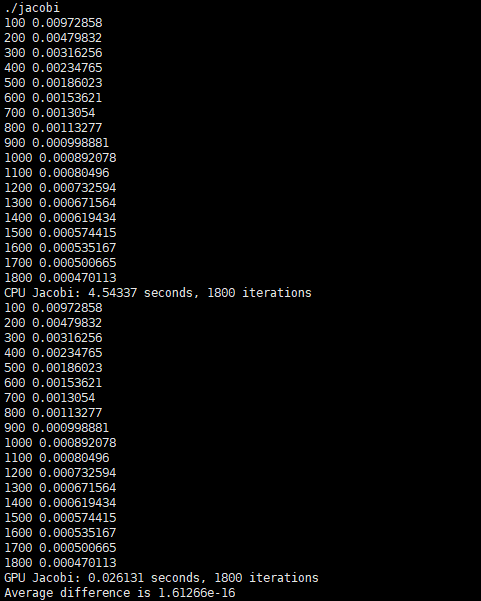
\includegraphics[width=0.8\linewidth]{fig/res2.PNG}
\end{figure}

\end{document}